\documentclass[a4paper,12pt,titlepage]{article}
\usepackage{graphicx}
\usepackage[hidelinks]{hyperref}
\usepackage{listings}
\usepackage{float}
\usepackage{pdflscape}
\usepackage{epstopdf}
\usepackage{rotating}
\usepackage[margin=1in]{geometry}
\usepackage[utf8]{inputenc}
\usepackage[english]{babel}
\usepackage[nottoc]{tocbibind}
\DeclareGraphicsExtensions{.png,.eps,.jpg}
\usepackage{amsmath}
\DeclareRobustCommand{\rchi}{{\mathpalette\irchi\relax}}
\newcommand{\irchi}[2]{\raisebox{\depth}{$#1\chi$}} % inner command, used by \rchi

\begin{document}
%\title and intnro
\begin{titlepage}
	\begin{center}
		
		\begin{figure}[t]
			\centering
			
\includegraphics[width=450px]{./Graphics/KPTH_Logo}
		\end{figure}		
		
		\textbf{\LARGE Gynaecological Patient Information
		management System:}
		
		\vspace{1 cm}
	    \textbf{\LARGE \\Master Documentation}
		
		\vspace{1 cm}
		\LARGE{\textbf{Team Pentec: }}
		

		\begin{flushright} \large
			
			Ruth Ojo 12042804\newline
			Liz Joseph 10075268\newline
			Trevor Austin 11310856\newline
			Maria Qumayo 29461775\newline
			Lindelo Mapumulo 12002862\newline
		\end{flushright}
		
				\vspace{1 cm}
				\centering
				
\includegraphics[width=150px]{./Graphics/Pentec_Logo.png}

		
		
		{\LARGE Final Version}
		\\
		{\large \today}		
		
		
	\end{center}
\end{titlepage}

\tableofcontents
\newpage

%\Intro
\section{Vision and Scope}
\subsubsection{Project Background}
The system should allow data to be entered by medical students, junior doctors 
and  registrars  (specialists  in  training)  working  in  the  department.  People  who 
enter  data  should  have  usernames  and  passwords  (student  numbers  and 
HPCSA registration numbers can be used) and they should only be able to enter 
information  and  should  not  have  access  to  data.  They  should  be  able  to  enter 
data using smartphones, tablets or personal computers in an environment where 
the hospital is not computerized and computers are not available in the hospital 
for this purpose. \par 

For purposes  of  entering  data  smartphone and  tablet applications (apple  and 
android)  should be  developed  to  allow  smartphone  and  tablet  access  to  the 
system. \par

The data should be securely stored on a site on the Website of the University of 
Pretoria. \par

Data  will  be  entered  into  the  system  by  different  employees  working  in  the 
Department  of  Obstetrics  \&  Gynaecology  at  the  Kalafong  Provincial  Tertiary 
Hospital. \par

Data of patients entered should include both the patient’s hospital number as well 
as RSA Identity number. \par

The  possibility  of  linking  this  system  to  that  of  the  National  Health  Laboratory 
System (NHLS) should be investigated to make it possible to access laboratory 
results through this system. The NHLS has an online accessibility. \par

The  administrator  of  the  system  should  have  access  to  all  relevant  data.  The 
different levels and specifications of data output will be defined upfront and the 
ability should exist to add or edit these specifications as required. \par

Patient  information  and  data  are  highly  confidential  and  the  website  and 
information  should  be  secure.  All  users  will  have  to  use  a  username  and 
password. Medical students can use University of Pretoria student numbers and 
medical interns, medical officers and registrars can use their Health Professions 
Council  of  South  Africa  (HPCSA)  unique  registration  numbers.  Doctors  and 
students  rotate  through  the  department  for  different  time  periods  and  the 
usernames and passwords should expire depending on the different categories. 
Students  rotate  for  four  weeks,  medical  interns  for  four  months  and medical 
officers and registrars  for  up  to  five  years.  Administrative  staff  and  consultants 
are more permanent and for security reasons should perhaps update information 
yearly. \par

\subsubsection{Project Vision}
\subsubsection{Project Scope}
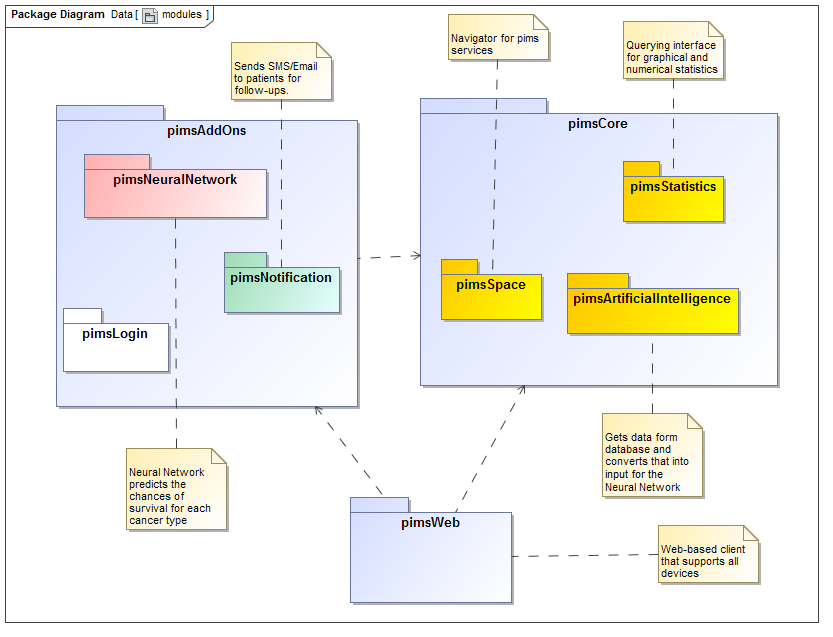
\includegraphics[width=\linewidth]{./Graphics/globalImages/modules}
%------------------------------------------------------------------------------------------------Functional Requirements------------------------------------------------------------------------------------------------%
\section{Application requirements and design}

\section{PIMS Login Module}
This module is responsible for allowing a user to login into and Logout out of Pentec Patient Information Management System. A user should login with the credentials they were assigned upon registration. If the user is not assigned a username then an exception is thrown and the user is redirected to the login page. \par 

To avoid "Spambots", a CAPTCHA challenge is used. 

\subsection{Scope}
The scope is shown in the use case diagram below: \par
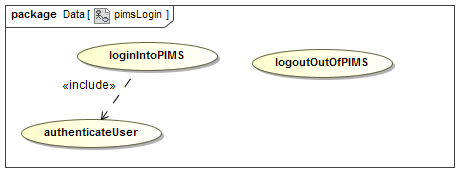
\includegraphics[width=0.75\linewidth]{./Graphics/pimsLogin/pimsLogin}

\subsection{Use cases}
	\subsubsection{loginToPIMS:} 
		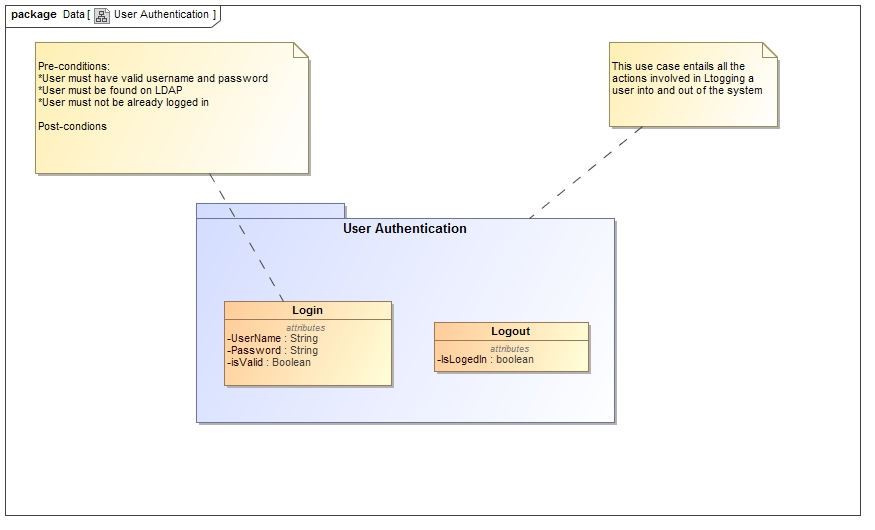
\includegraphics[width=0.7\linewidth]{./Graphics/Login}
	\subsubsection{logoutOfPIMS:}  
		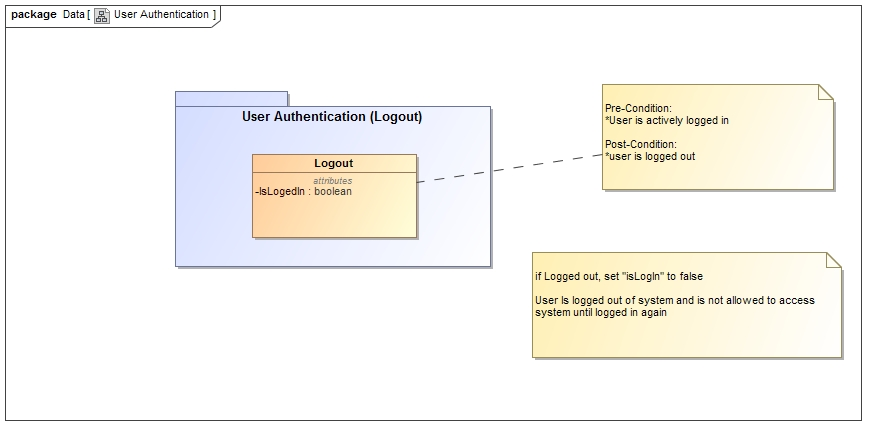
\includegraphics[width=0.7\linewidth]{./Graphics/Logout}



\subsection{PIMS Statistics Module}
This module is responsible for displaying statistics from the database. The user has an option to choose the type of graph (either a bar chart or line graph). \par 

\subsubsection{Scope}
The scope is shown in the use case diagram below: \par
\begin{figure}[H]
	\centerline{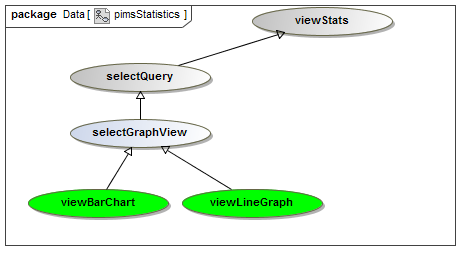
\includegraphics[width=0.7\linewidth]{./Functional_Requirements/Graphics/pimsStats/pimsStatistics}}
	\caption{PIMS statistics module scope}
\end{figure}

\subsubsection{Use cases}
\begin{description}

	\item{\textbf{viewStats -- [priority: critical]}} This use case is a generic version of all statistics to be obtained. Sub-use cases follow the same contract, but return different data.
	\begin{description}
		\item{\textbf{Service Contract}} The generic service contract for all statistics is shown below.
		\begin{figure}[H]
			\centerline{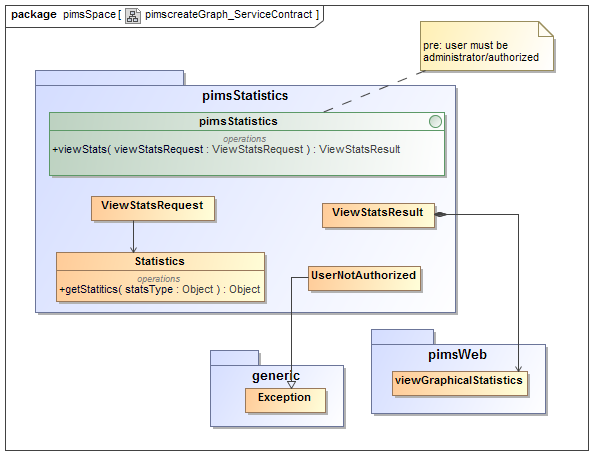
\includegraphics[width=0.7\linewidth]{./Functional_Requirements/Graphics/pimsStats/pimscreateGraph_ServiceContract}}
			\caption{Service contract for viewStats}
		\end{figure}
	\end{description}
		\begin{description}
		\item{\textbf{Process Specification}} The generic process specification for all statistics is shown below.
		\begin{figure}[H]
			\centerline{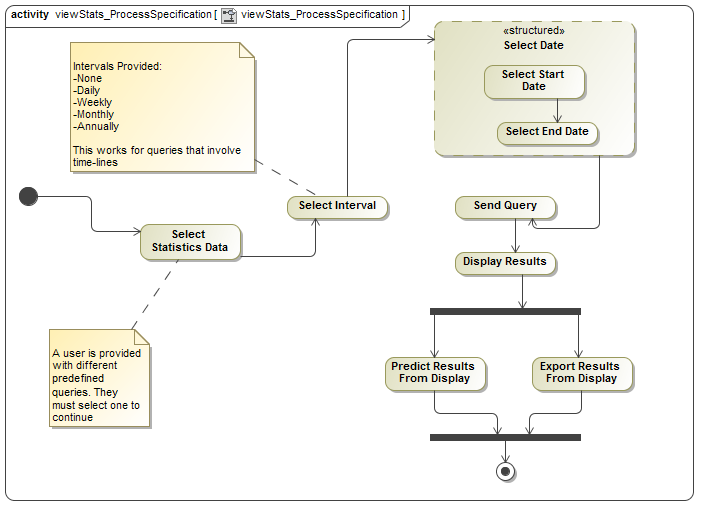
\includegraphics[width=0.7\linewidth]{./Functional_Requirements/Graphics/pimsStats/viewStats_ProcessSpecification}}
			\caption{Process specification for viewStats}
		\end{figure}
	\end{description}
	
		\item{\textbf{createGraph -- [priority: critical]}} This use case creates and displays a graph. This graph can be viewed by the client or downloaded for record keeping.
	
\end{description}

\newpage
\subsection{PIMS Artificial Intelligence Module}
This module is responsible for predicting the chances of survival for each cancer type. Parameters for each patient are considered to compute this prediction. These parameters are converted into a single value that will be used by the PIMS Neural Network Module as input. \par 

\subsubsection{Scope}
The scope is shown in the use case diagram below: \par
\begin{figure}[H]
\centerline{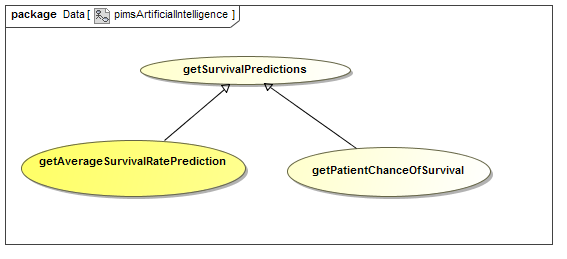
\includegraphics[width=0.75\linewidth]{./Functional_Requirements/Graphics/pimsAI/pimsArtificialIntelligence}}
\caption{The global scope for PIMS Artificial Intelligence Module}
\end{figure}

\subsubsection{Use cases}
\begin{description}

	\item{\textbf{getAverageSurvivalRatePrediction -- [priority: critical]}}
	\begin{description}
		\item{\textbf{Service Contract}} The generic service contract
		\begin{figure}[H]
			\centerline{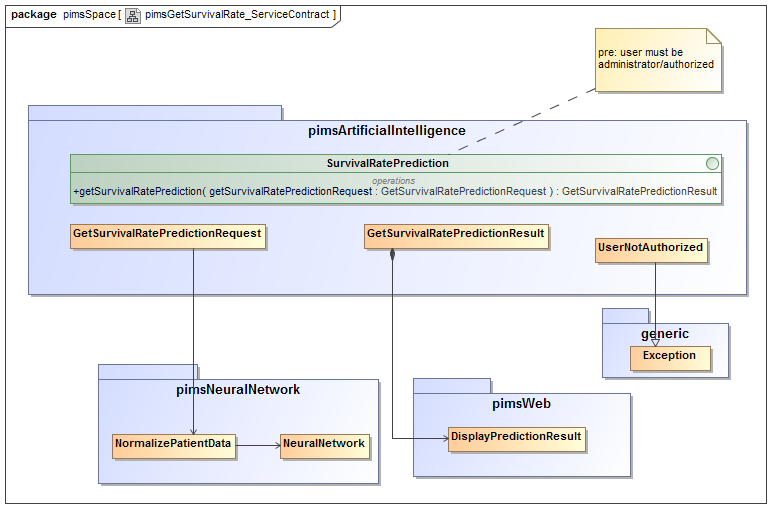
\includegraphics[width=0.8\linewidth]{./Functional_Requirements/Graphics/pimsAI/pimsGetSurvivalRate_ServiceContract}}
			\caption{Service contract for getAverageSurvivalRatePrediction}
		\end{figure}
	\end{description}
	
		\item{\textbf{getPatientChanceOfSurvival -- [priority: critical]}}
	\begin{description}
		\item{\textbf{Service Contract}} The generic service contract
		\begin{figure}[H]
			\centerline{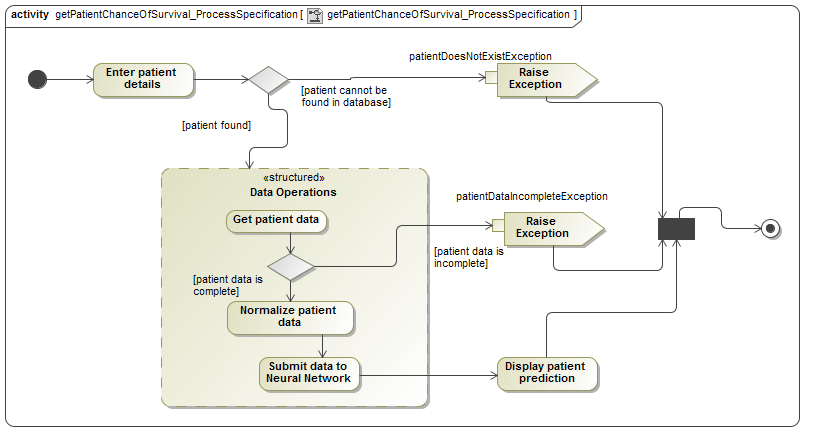
\includegraphics[width=0.9\linewidth]{./Functional_Requirements/Graphics/pimsAI/getPatientChanceOfSurvival_ProcessSpecification}}
			\caption{Process specification for Service contract for getPatientChanceOfSurvival}
		\end{figure}
	\end{description}
\end{description}

	\subsubsection{Neural Network Training}
	Patient data was analysed for possible risk factors for cancer susceptibility. These risk factors are:
	\begin{itemize} %Lindelo you can add the paramters used and explain how you normalized each one with justifications
		\item Age - No normalization was required for this field. However, decimal scaling was used for the age. Patients are expected to be within the age range of [16 - 100] so the age is scaled-down to two decimal places.
		\item HIV status - Is a binary field (either negative or positive). Negative HIV statuses were given the numerical equivalent of 0.9 while a positive status holds 0.1.
		\item CD4 count (If HIV status is positive) - If the patient is HIV negative, the numerical values becomes 0.9998. Otherwise, decimal scaling (4 places down) is used since the CD4 range is 0 - 1500.  
		\item Figo Stage - Since this value is neither binary nor numeric, the number of figo stages determines how the patient's stage is normalized. If there are n stages then the kth stage gets the numerical equivalent of : \(\frac{k-stage}{n}\)
		\item Site of distant metastase - Same as the Figo stage. 
		\item Histology - Also uses the same concept as Figo stage.
		\item Differentiation - Also uses the same concept as Figo stage.
		\item Primary treatment -  Also uses the same concept as Figo stage.
		\item Type of surgery - Also uses the same concept as Figo stage.
		\item Type of radiotherapy - Also uses the same concept as Figo stage.
		\item Response to treatment - Also uses the same concept as Figo stage.
		\item Relapse - Also uses the same concept as Figo stage.
		\item Last known vital status - Also uses the same concept as Figo stage.
		
	\end{itemize}
	
	The Neural Network makes use of the back-propagation algorithm for the purpose of learning.

	\begin{itemize}
		\item The equations used for the neural network are as follows:
		\begin{itemize}
			\item Input Function:
			 \[net =\sum_{i=1}^{n} {x_i} {w_i}\]
			 
			 \item Hidden layer Input Function:
			  \[net_{y_i} =\sum_{i=1}^{I + 1} {z_i}{w_ji}\]
			  
			  \item Hidden layer Sigmoid Activation function:
			  
			  \[y_j =\frac{1}{1 + {e}^{-net_{y_j}}}\]
			  
			   \item Output layer Input Function:
			  
			  \[net_{o_k} =\sum_{j=1}^{I + 1} {y_j}{w_kj}\]
			  
			  \item Output layer Sigmoid Activation function:
			  
			  \[o_k =\frac{1}{1 + {e}^{-net_{o_k}}}\]			  
			
			\item Sigmoid Activation function: \[f(net) =\frac{1}{1 + {e}^{-net}}\]
			
			\item Training error: \[Error =(t_k - o_k)\]
			
			

		\end{itemize}
		
		\begin{itemize}
		\item The equations used for the back propagation phase are as follows:
			\begin{itemize}
				\item Output layer error propagation:
				 \[\delta_{o_k} = -(t_k - O_k)(1 - O_k)O_k\]
				 
				 \item Output layer weights propagation:
				 \[w_{k_j}{o_k} \mathrel{+}= -(\delta_{o_k}y_j\]

				 \item Hidden layer error propagation:
				 \[\delta_{y_j} = -(w_{k_j} \delta_{o_k} (1-y_j)y_j\]				 
				 
				 \item Hidden layer weights propagation:
				 \[v_{j_i} \mathrel{+}= \delta_{y_j}z_i\]
				 

			\end{itemize}
		\end{itemize}
	
	\end{itemize}
	
	
	\subsubsection{Neural Network Testing}
	When testing the network, a the critical cancer parameters are normalized given a patient name. When classifying the patient as likely to survive or die form cancer the principles of a statistical probability density function, ${\rchi^2}$-distribution are applied; wherein the null hypothesis is \setlength{\thinmuskip}{0mu} (\textbf{$H_0$}):
	\begin{itemize}
		\item A patient is likely to survive cancer
	\end{itemize}
	 in order to obtain a confidence interval for the survival prognosis. A 50\% significance level is used for the confidence interval; such that 50\% of the time, the output node value is likely to be a false positive and as for the other percentage, one can be confident in it as being accurate. The choice of the application of the ${\rchi^2}$-distribution is plainly for it's simplicity and it is a well known probability density function. The choice of the confidence interval was aided by the application of artificial neural networks in survival analysis when compared with other survival analysis statistical models \cite{BeyondtheCoxmodel}.
	
	\begin{itemize}
		\item The below ${\rchi^2}$-distribution formulas are used:
		
		\begin{itemize}
			\item Probability: \footnote{\textit{n} is the number of patients to test, \textit{E} is the target, \textit{O} is the output node value, \textit{k is the individual patient}}
			\[\chi^2=\frac{1}{d}\sum_{k=1}^{n} \frac{(O_k - E_k)^2}{E_k}\]
			\item Confidence interval: \footnote{\textit{s} is the mean square error}
			\[\pm    \frac{(n-1) \times s^2}{\chi^2_{\frac{\alpha}{2}} \times (n-1)}\]
			\item Degrees of freedom: \[(n-1)\]
		\end{itemize}
		\item The ${\rchi^2}$-distribution table of critical values will be used to test (\textbf{$H_0$})		
			\begin{figure}[H]
			\centerline{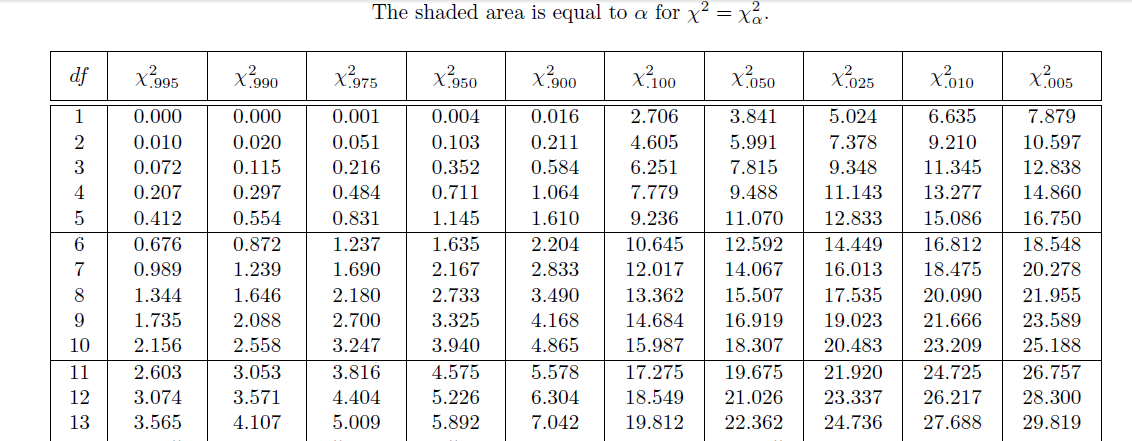
\includegraphics[width=0.8\linewidth]{./Functional_Requirements/Graphics/pimsAI/Chi_image}}
			\caption{Snippet of Chi-squared distribution critical value table}
		\end{figure}
		
		
	\end{itemize}


\newpage
\subsection{PIMS Notification Module}
This module is responsible for sending email/SMS notifications to a patient. This email/text message could be a reminder to a patient about follow up visits to the doctor. \par 

\subsubsection{Scope}
The scope is shown in the use case diagram below: \par
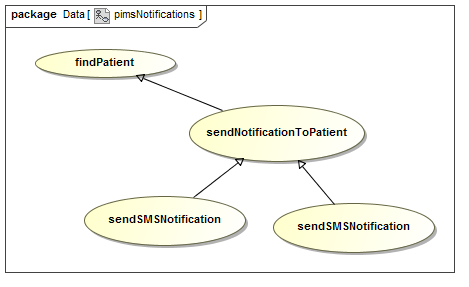
\includegraphics[width=0.75\linewidth]{./Graphics/pimsNotification/pimsNotifications}

\subsubsection{Use cases}
\begin{description}
	\item{\textbf{findPatient -- priority: nice-to-have}}
	This use case is to cater for the retrieval of a patient ID/name form the database so as to obtain the contact details of the patient, if any.
	\begin{description}
		\item{\textbf{Service Contract}} The service contract for findPatient is shown below.
		\begin{figure}[h!]
			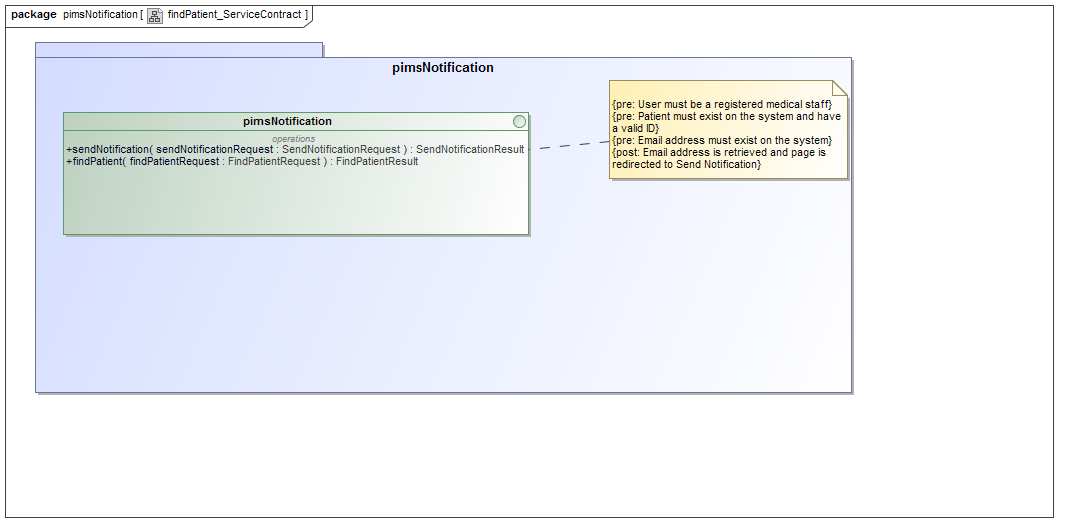
\includegraphics[width=\linewidth]{./Graphics/pimsNotification/findPatient_ServiceContract}
		\end{figure}
	\end{description}	
	
	\item{\textbf{sendSMSNotification -- priority: nice-to-have}}
	This use case is to cater for the sending of a follow-up notification message via SMS depending on whether or not the patient has a cellphone number that is stored on the system.
	\item{\textbf{sendEmailNotification -- priority: nice-to-have}}
	This use case is to cater for the sending of a follow-up notification message via E-mail depending on whether or not the patient has an email address that is stored on the system.
	
	\begin{description}
		\item{\textbf{Service Contract}} The service contract for sendSMSNotification and  sendEmailNotification is shown below.
		\begin{figure}[h!]
			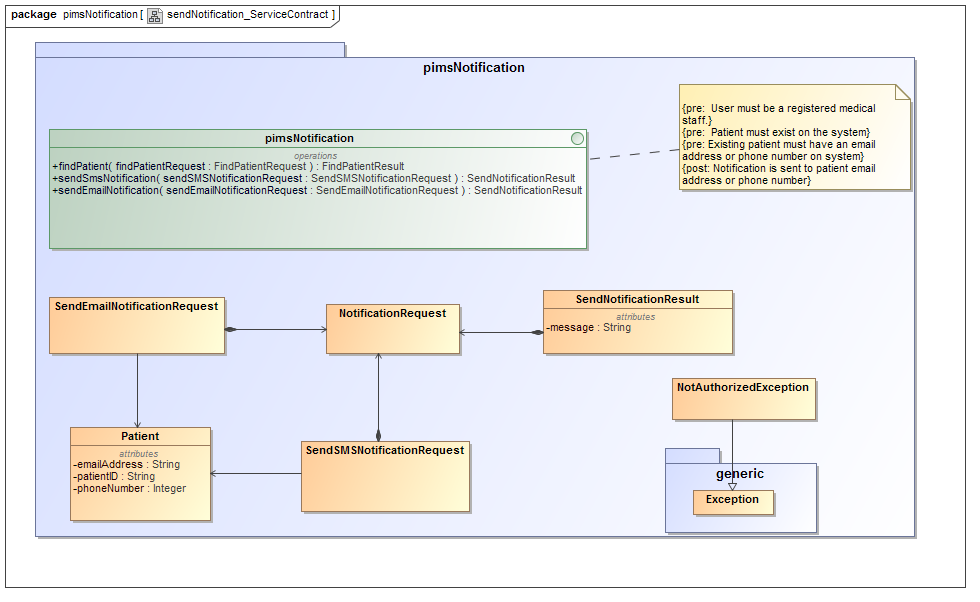
\includegraphics[width=\linewidth]{./Graphics/pimsNotification/sendNotificatioServiceContract}
		\end{figure}
	\end{description}		
	
\end{description}
\subsection{PIMS Space Module}
This module is responsible for providing all the core functionality of Patient Information Management System. The front-end component displays all the available services to the user. \par 

\subsubsection{Scope}
The scope is shown in the use case diagram below: \par
		\begin{figure}[H]
			\centerline{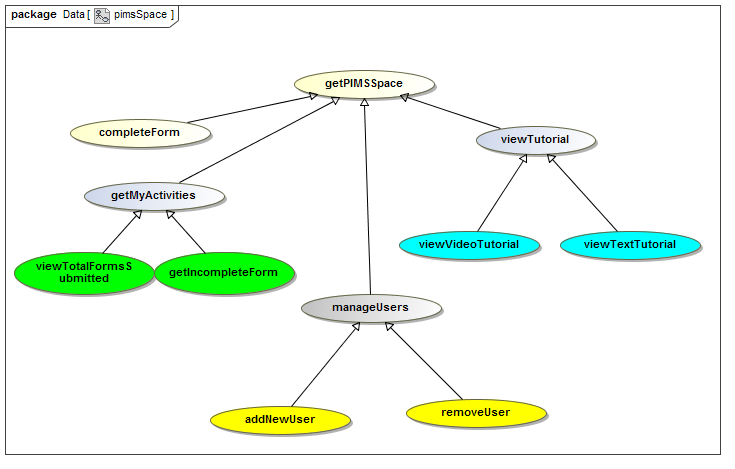
\includegraphics[width=0.75\linewidth]{./Functional_Requirements/Graphics/pimsSpace/pimsSpace}}
			\caption{Scope for PIMS Space Module}
		\end{figure}

\subsubsection{Use cases}
\begin{description}
	\item{\textbf{getPIMSSpace:}}
		\begin{description}
		\item{\textbf{Service Contract}}
		\begin{figure}[H]
			\centerline{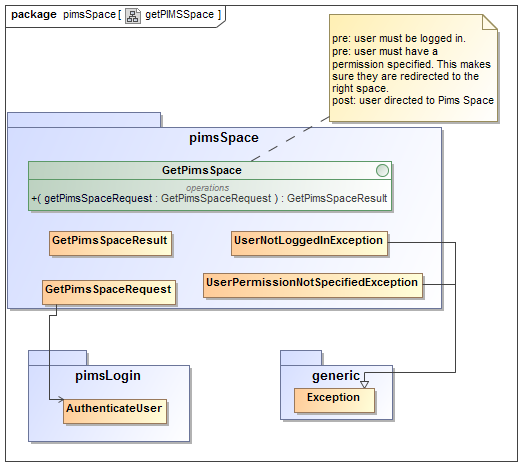
\includegraphics[width=0.7\linewidth]{./Functional_Requirements/Graphics/pimsSpace/getPIMSSpace}}
			\caption{Service contract for getPIMSSpace}
		\end{figure}
	\end{description} 
	\item{completeForm:}
			\begin{description}
		\item{\textbf{Service Contract}}
		\begin{figure}[H]
			\centerline{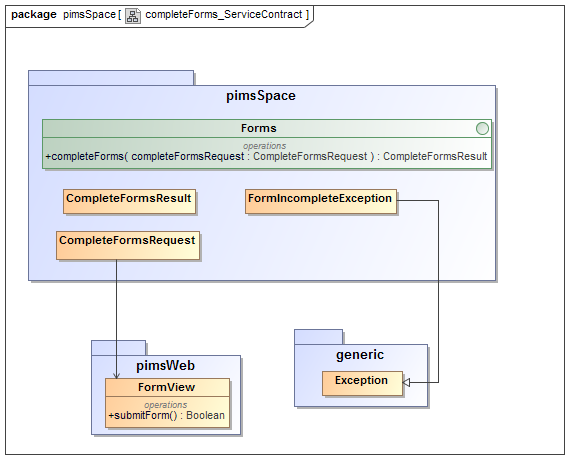
\includegraphics[width=0.7\linewidth]{./Functional_Requirements/Graphics/pimsSpace/completeForms_ServiceContract}}
			\caption{Service contract for completeForm}
		\end{figure}
	\end{description} 
	\item{viewTutorial:}
	\item{addNewUser:}
			\begin{description}
		\item{\textbf{Service Contract}}
		\begin{figure}[H]
			\centerline{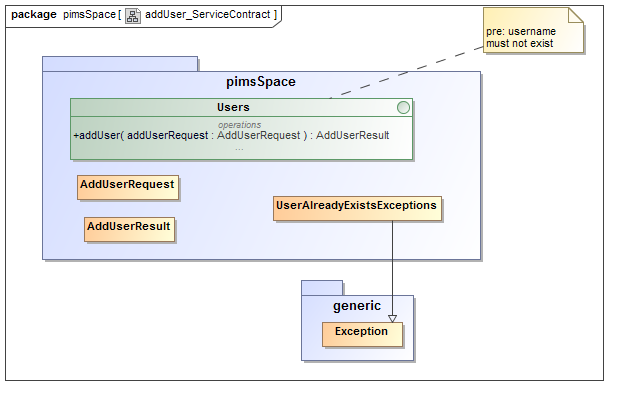
\includegraphics[width=0.7\linewidth]{./Functional_Requirements/Graphics/pimsSpace/addUser_ServiceContract}}
			\caption{Service contract for addNewUser}
		\end{figure}
	\end{description} 
	\item{removeUser:}
			\begin{description}
		\item{\textbf{Service Contract}}
		\begin{figure}[H]
			\centerline{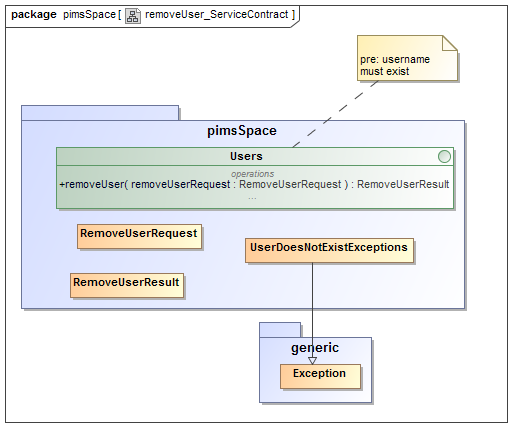
\includegraphics[width=0.7\linewidth]{./Functional_Requirements/Graphics/pimsSpace/removeUser_ServiceContract}}
			\caption{Service contract for removeUser}
		\end{figure}
	\end{description} 
	\item{viewTotalFormSubmitted:} 
	\item{getIncompleteForm:}
\end{description}


%------------------------------------------------------------------------------------------------Architectural Requirements------------------------------------------------------------------------------------------%
\newpage
\section{Architectural requirements}
	%\subsection{Architectural Scope} %Maria
	%

%Persistence
\subsubsection{Persistence}

\subsubsection{Reporting}
			 
%Process execution
\subsubsection{Process execution}


	
	\subsection{Access and integration requirements}
			\subsubsection{Human access channels}	
				Human Access Channels are all the various ways a user may interact with and access the PIMS.

\begin{enumerate}
	\item Mobile Phone:
	\begin{itemize}
		\item This mode of access will allow for better mobility and portability as the user can fill in information as they perform procedures. The user will have to use their own data to access the system.
	\end{itemize}
	\item Tablet:
	\begin{itemize}
		\item This mode of access, same as the mobile phone, will also for mobility and portability.
	\end{itemize}
	
	\item Desktop Computer:
	\begin{itemize}
		\item This will be the least common way for the user to access the PIMS, as the Hospital does not have a centralized computer.
	\end{itemize}
	\item Laptop:
	\begin{itemize}
		\item This mode of access is more portable than the desktop computer.
		\item The user will have to make use of a modem to access the Internet as the Hospital does not Wi-Fi access.
	\end{itemize}

\end{enumerate} 
			\subsubsection{System access channels}
				System Access Channels are the means by which other systems will access the services offered by the Kalafong PIMS.
At the moment, no system access channels are required.	
			\subsubsection{Integration channels}
				The PIMS will need to be integrated with:
\begin{itemize}
	\item The NHLS website in order to retrieve diagnostic codes form the website
		\begin{itemize}
			\item This functionality is to be executed at a later stage, outside the scope of the COS 301 Main Project.
	\item The University of Pretoria website by linking the two websites
	\item The existing departmental Microsoft Access database
	\item The individual datasets that will be part of the system
\end{itemize}

				
	\newpage			
 	\subsection{Quality requirements} 	
		%\underline{\textbf{Critical Quality Requirements}}	
		\subsubsection{Usability ( - priority:critical)} \label{sec:usability}
			%Lindelo - Usability
			\subsection{Usability}
\subsubsection{Description}
This ensures that a user will be able to use the system, with ease. The system should provide support to the user.
\subsubsection{Justification}
Patient information management system is user-oriented. How the users interact with the system is a critical, and this should be done with little to no effort. The system should appear easy to use and should not, at any point, baffle the users. 
\subsubsection{Mechanism}
	\begin{enumerate}
		\item Strategy:
		
		 	\begin{itemize}
		 	\item A tutorial on how the patient information management system works. A user can be initiated into the system, the 					  first time they use it. Or they can enable the tutorial until they're familiar with the functionality.
		 	\item Enable the user to troubleshoot their problems. Frequently asked questions or frequent problems could assist 						with this aspect.  A user will be provided with predefined help options such that they will not need to contact 					the system's administrator, for assistance.
		 	\item Provide descriptive headings that make navigation easier. Headings should not be ambiguous. A user should 						  know what to expect when they select a certain heading.
		 	\item Error signals should be displayed to the user, if some user-inflicted error occurs. The necessary steps to 		                  rectify this problem must be provided.
		 	\item A user should be able to undo their action, should they be aware of their mistake.
		 	\end{itemize}
		 	
		\item Architectural Pattern(s):
		
			\begin{itemize}
			\item Model-View-Controller: This separates the user interface from the rest of the system (Bass and John). A user 		                  should only interact with a simple interface that was designed for them. This is describable for patient         					information management system because the users don't necessary have an adept understanding of the lower     		                levels of the system.
			\end{itemize}
	\end{enumerate}
			
		\subsubsection{Scalability ( - priority:critical)} \label{sec:scalability}
			%Ruth - Scalability
				\subsubsection*{Description}
	Scalability is an essential aspect of a system and is the ability of a system to be easily enlarged in order to accommodate a growing amount of work.
	\subsubsection*{Justification}
	 The PIMS should allow for hundreds of concurrent users, as such the system must be able to handle such a number without breaking down or reducing performance.
	\subsubsection*{Mechanism}
		\begin{enumerate}
			\item Strategy:
			\begin{itemize}
			\item Clustering: using more resources by running many instances of the application over a cluster of servers or instances, to ensure system resources are not strained by a high workload.
			
			\item Efficient use of storage: data storage can be efficiently used through compression of the data (reducing data size to make room for more) paging (ensuring that primary storage is used only for more crucial data) as well as de-fragmentation (organizing the data into continuous fragments and free more storage space).
			by ensuring that no data duplications occur, storage space can be conserved, thus the load on system resources will be reduced.
			\item Efficient persistence: through indexing and query optimization, the amount of system power used to persist a database will be reduced, as data retrieval will be quicker and costly queries will be done without, thus also reducing system load. In addition, connections can be grouped and accessed via a central channel in order to aid persistent storage to the database.
			
			\item Load Balancing: by spreading the systems load across time or across resources the load on the system can be distributed, therefore no system resource will be heavily strained. In the case that the limit for a server has been reached, a new instance or so will have to be created in order to handle the number of increasing requests. On the other hand, if the usage of a server is way below the capacity, the number of instances will have to be reduced.
			
			\item Caching: to ensure no duplication or repeated retrieval of frequent objects or queries; a separate module can facilitate caching; thus system resources will not be used up unnecessarily.
			 \end{itemize}

		\end{enumerate}
			
		\subsubsection{Reliability and Availability ( - priority:critical)} \label{sec:reliabilityavailability}
			%Ruth - Reliability and Availability
			
\subsubsection*{Description}
The PIMS should be accessible at almost all times, in particular during the peak operational hours of the hospital. This accessibility will be limited to the hospital network only, so as to ensure no information can be changed without approval.
		
\subsubsection*{Justification}
The reliability and availability requirements are very important seeing as the information to be kept on the system is highly valuable to the medical staff, as the need up-to-date information concerning the patients they are dealing with (lives could be at risk).							 
With this in mind, only a downtime of less than 2 hours, at most twice a month will be allowed, so as too allow for the medical staff to maximally use the system.
A high reliability rate is recommended to ensure that users do not encounter any errors and/or data corruption in their use of the system. The only leeway that will be given for errors, is to have at most one.
	
	
\subsubsection*{Mechanism}	
\begin{enumerate}
\item Strategy:
	\begin{itemize}
		\item Clustering: using more resources by running many instances of the application over a cluster of servers or instances; therefore if any server should fail, the reliability and availability of the system will not be compromised.
		\item For reading from and writing to the database, we will ensure that no parallel updates are possible through enforcing the use of a single object to stream all database transactions; thus reducing inaccuracy that would be a result of data redundancy.		 
		\item Use of more resources: This would heavily reduce system downtime, as a temporary server can be run while the other is maintained.
\end{itemize}
					
\end{enumerate}

			
		\subsubsection{Integrability ( - priority:critical)} \label{sec:integrability}
			%Maria - Integrability
			%Integratability
\subsubsection *{Description:}
	  The Patient Information Management System should be integrated with ease to the Universities website as well as the NHSA web site.
	 \subsubsection *{Justification:}
	   The Patient Information Management System is primarily designed for the kalafong medical staff and is required to be accessable on both the University's website and the NHSA website. For security perposes we limit it's intergaration to just these two sites.
	\subsection *{Mechanism:}
	\begin{enumerate}
		\item Strategy: \\\ The contracts based decoupling strategy is used to implement integrability and extensibility on the system by providing sections and different functionality between the back end system and the host site. 
	\end{enumerate}
		%\underline{\textbf{Important Quality Requirements}}
		
		\subsubsection{Security ( - priority:important)} \label{sec:security}
			%Lindelo - Security
			\subsection{Security}
\subsubsection{Description}
This is the most critical requirement for the patient information management system. Patient's information should not only be 
confidential, but levels of user authorisation must exist. The existing information should not be modifiable by users that have no 
access to the information; this also applies to outside intruders.
\subsubsection{Justification}
The whole system should not be penetrable by an intruder; the general public should not have access to any of the information about the patients. The system should also make sure that each user can only access the attributes that applies to them.
\subsubsection{Mechanism}
	\begin{enumerate}
		\item Strategy:
		
		 	\begin{itemize}
		 	\item Encryption: Patient data is confidential and should be encrypted. Not every patient has to be encrypted, but 
		 	the data should not imply to which patient it belongs to. The patient's personal information could be encrypted instead 			of all the attributes.
		 	\item Authorization: A user's access level and identity needs to be determined before they can access the system. 
		 	\item Store log information: Although this applies to audibility, it helps to know the nature of a security threat.   					If new threats are noted, more security features can be implemented.
		 	\end{itemize}

	\end{enumerate}		
		
		\subsubsection{Maintainability ( - priority:important)} \label{sec:maintainability}
			%Maria - Monitorabilty
			\subsubsection*{Description}  \label{sec:maintainability}
The PIMS should be easily Maintainable in future. Thus needs to be flexible and extensible.
		
\subsubsection*{Justification}
Software always needs new features or bug fixes. Maintainable software is easy to extend and fix, which encourages the software's uptake and use.
	
	
\subsubsection*{Mechanism}	
\begin{enumerate}
\item Strategy:
	\begin{itemize}
		\item Open-source resources: using open source resources to minimize update costs in the future.
		\item Iterative development and regular reviews: This will help us improve system quality.
		\item Prevention is better than cure: Here we get others(lecturers) to review your code, to make sure its clean.The cleaner our code, the cheapre it is to maintain.
		\item Version control:Thsi will help keep our code, tests and documentation up to date and synchronised. It will also help us keep track of progress.
		\item Documentation: Relevant documentation will help future developers understand the software and system as a whole.
\end{itemize}
					
\end{enumerate}
			
		\subsubsection{Monitorability/Auditability ( - priority:important)} \label{sec:auditability}
			%Maria - testability
			%Monitorability
	\subsubsection*{Description}
		Audititabily or Monitor-ability is a software review where one or more auditors/monitors who are not members of the software development and organization team conduct "An independent examination of the software product to assess compliance with specifications, standards, contractual agreements, functional requirements and other criteria according to the development specification. Software Monitor-ability and audiability is different from testing or peer reviews because they are done by personnel external to and independent of the software development organization.
	\subsubsection*{Justification}
	Although it is important for the PIMS to be monitorable, it is not crucial. It may be Monitored because of the following:
					\begin{itemize}
							\item Multiple and concurrent users, thus making it prone to various malfunctions.
							
							\item Form filling and Statistical quering needs to be done in real time at all times to ensure relevance of topics and subject matters.
							
							\item Sufficient feedback and updates of the site's state must be provided to the users.
							
							\item General software control and application usage..
						 \end{itemize}
	
	\subsubsection*{Mechanism}
		\begin{enumerate}
			\item Strategy:\\\\
			Auditability and monitor-ability will be achieved by allowing any third party software auditor or monitor support group reviewing the Buzz Space examining it specifically for the aspects of the functional requirements as given by the client. Information such as the systems state and processes in complaints with the specification given. One such auditor may be from a well-established organisation, for example Oracle’s PeopleSoft enterprise which is UP’s current used application.	
			
			
			 \item Pattern/Tools:\\\\
			 Tools like SMaRT, a workbench for reporting the monitor-ability of Service Level Agreements for software services such as Buzz Space may be used. SMaRT aims to clearly identify the service level the service level commitments established between service requesters and providers. This monitoring infrastructure can be used with mechanical support groups in the form of a SMaRT Workbench Eclipse IDE plug-in for reporting on the monitor-ability of Service Level Agreements.
			 
		\end{enumerate}

			
		\subsubsection{Testability ( - priority:important)} \label{sec:testability}
			%testability
	\subsubsection*{Description}
		Testability is a measure of how well system or components allow you to create test criteria and execute tests to determine if the criteria (pre and post conditions)are met. Testability allows faults in a system to be isolated in a timely and effective manner.
		
		
	\subsubsection*{Justification}
	It is extremely important to conduct test cases for every component that will be intergrated or incorporated into PIMS. This ensures consistency in the system,and enables faults and/or loopholes to be picked up and resolved in good time.
	
	\subsubsection*{Mechanism}
		\begin{enumerate}
			\item Strategy:\\\\
		\begin{itemize}
			\item Unit testing: Unit testing and integration testing will be conducted using moch and unit.js
			\item	White-box tests internal structures or workings of an application. This requires the explicit knowledge of the internal workings of the PIMS.
		\end{itemize}
		
		
			 \item Pattern:\\\\
		 \begin{itemize}
			\item	Layering:  Simplify testability since high level issues will be separated from low level issues. This level of granularity makes the system to be easily testable on every layer separately.
			\item Model View Controller: The PIMS model will be separate from the view and the controller, so that it is simpler to have separate test criteria testing different cases. This separation simplifies the development cycle since the model, view or the controller could be tested independently. 
		\end{itemize}
\end{enumerate}
		
		\subsubsection{Performance ( - priority:important)} \label{sec:performance}
			\subsubsection*{Description}
The PIMS should be easily Maintainable in future. Thus needs to be flexible and extensible.
		
\subsubsection*{Justification}
Software always needs new features or bug fixes. Maintainable software is easy to extend and fix, which encourages the software's uptake and use.
	
	
\subsubsection*{Mechanism}	
\begin{enumerate}
\item Strategy:
	\begin{itemize}
		\item Open-source resources: using open source resources to minimize update costs in the future.
		\item Iterative development and regular reviews: This will help us improve system quality.
		\item Prevention is better than cure: Here we get others(lecturers) to review your code, to make sure its clean.The cleaner our code, the cheapre it is to maintain.
		\item Version control:Thsi will help keep our code, tests and documentation up to date and synchronised. It will also help us keep track of progress.
		\item Documentation: Relevant documentation will help future developers understand the software and system as a whole.
\end{itemize}
					
\end{enumerate}
			
	\newpage
	\subsection{Architectural responsibilities}
		The architectural responsibilities for the PIMS include:
\begin{enumerate}
	\item Logging in and out of users of the system
	\item User authentication
	\item Appropriate authorization for  access of resources
	\item form generation through JSON Schemas
	\item statistics calculation and graph generation
	\item a web and mobile access channel
	\item the persisting and accessing of patient information
	\item sending notification messages by email or SMS
	\item integration with University of Pretoria website
	\item logging of all operations on the website
	\item cancer survival rate predictions through a feed-forward neural network
\end{enumerate}
		
	\newpage	
	\subsection{Architecture constraints}
		\begin{itemize}
	\item The architecture is largely constrained to node.js and MongoDB.
	\item Due to the nature of node.js' single-threaded processing there may be an impact on performance, but this will be balanced out with the use of other performance-driven technologies, such as MongoDB.
\end{itemize}

\subsection{Data exchange format}
\begin{itemize}
	\item The transfer of data between the server and client side as well as from the database will primarily be in JSON format, particularly due to the nature of the MongoDB database data format.
\end{itemize}

\subsection{Neural Network}
\begin{itemize}
	\item The operation of the feed-forward neural network is to allow for background calculations that must be propagated in a user-friendly and eye-pleasing manner. As a result, the neural network must have not only a back-end for calculation but a front-end aspect as well. An nom Neural Network package that caters for browsers is used to cater for this.
\end{itemize}



%----------------------------------------------------
\newpage
\section{Architectural Patterns and Styles}
	\subsection{Model-View-Controller (MVC)}
	%Lindelo - MVC
	
Model-View-Controller is an architectural pattern that divides software applications into three interconnected parts. \\ \par
The controller is responsible for translating requests in to responses (Nadel, 2012). The controller 'inserts' the response back into the view, which could be html or it's equivalents. \par
The view translates the response, from the controller, into a visual format for the client (Nadel, 2012). The view also sends requests to the controller. \par
The model's task is to maintain state and give methods for changing this state. Typically, this layer can be decomposed to:
\begin{itemize}
\item Service layer - provides high-level logic for dependent parts of an application.
\item Data access layer - services objects invoke this layer, which provides provides access to the persistence layer.
\item Value object layer - provides data-oriented representations of terminal nodes in the model hierarchy.
\end{itemize}


\newpage	
\section{Architectural Design}	
	\subsection{Technologies}
		\subsection{Platform}
\begin{itemize}
		\item Java EE
\end{itemize}


\subsection{Frameworks}
\begin{itemize}
		\item Java Server Faces
\end{itemize}

\subsection{Operating System}
\begin{itemize}
		\item Linux
\end{itemize}
	
	
\subsection{Databases}
\subsubsection{Relational Databases}
\begin{itemize}
	\item MySQL Database
\end{itemize}
	

\subsection{Object Relational Mappers}
\begin{itemize}
	\item JPQL
\end{itemize}

\subsection{Languages}
\subsubsection{Programming Languages}
\begin{itemize}
	\item JavaScript	
	\item Java
\end{itemize}

\subsubsection{Mark-up Languages}
\begin{itemize}
	\item HTML
\end{itemize}


\subsection{Application Servers}
\begin{itemize}
	\item GlassFish Server
	\item Tomcat
\end{itemize}

\subsection{Dependency Management}
\begin{itemize}
	\item Apache Maven
\end{itemize}

\subsection{Web Services}
\begin{itemize}
	\item SOAP-based
\end{itemize} 


\subsection{APIs}
\begin{itemize}
	\item Java Persistence API
\end{itemize}

\begin{itemize}
	\item JAX-RS RESTful web services
\end{itemize}

\begin{itemize}
	\item JAX-WS web service endpoints
\end{itemize}

\begin{itemize}
	\item Java Persistence API entities
\end{itemize}

\begin{itemize}
	\item The Java Database Connectivity API (JDBC)
\end{itemize}

\begin{itemize}
	\item The Java Persistence API
\end{itemize}

\begin{itemize}
	\item The Java EE Connector Architecture
\end{itemize}

\begin{itemize}
	\item The Java Transaction API (JTA)
\end{itemize}


\subsection{Others}
\begin{itemize}
	\item AJAX
\end{itemize}

\begin{itemize}
	\item Servlets
\end{itemize}

\begin{itemize}
	\item Java Server Pages
\end{itemize}


\begin{itemize}
	\item JavaServer Faces
\end{itemize}

\begin{itemize}
	\item JavaServer Faces Facelets
\end{itemize}

\begin{itemize}
	\item Enterprise JavaBeans (enterprise bean) components
\end{itemize}

\begin{itemize}
	\item Java EE managed beans
\end{itemize}


\section{Recommended Technologies}
\subsection{Databases}
\subsubsection{Object Relational Databases}
\begin{itemize}
	\item Postgresql
\end{itemize}

\subsubsection{NoSQL Databases}
\begin{itemize}
	\item Neo4j
	\item MongoDB
\end{itemize}

\subsection{Object Data Mappers}
To cater for the use of NoSQL Databases
\begin{itemize}
	\item Hibernate OGM
\end{itemize}

	\newpage	
	\subsection{Tactics and Strategies Addressing Quality Requirements}
		\subsubsection*{Scalability and Performance}
	\begin{itemize}
		\item Optimize repeated processes.
		\item Reuse resources and results.
		\item Reduce contention by replicating frequently used resources.
		\item Clustering.
		\item Efficient use of storage.
		\item Load Balancing.
		\item Caching.
		\item Use REST (Representational State Transfer) to make BuzzSpace into a scalable web service.
	\end{itemize}	
\subsubsection*{Security}
	\begin{itemize}
		\item Authenticate users by requesting username and password when interaction with the system begins.
		\item Authorize users checking if a user has the rights to access and modify either data or services.
		\item Encryption to maintain confidentiality of data.
		\item Input Validation to detect malicious attacks.
		\item Auditing and logging for identifying and recovering from attacks.
	\end{itemize}	
\subsubsection*{Usability}
	\begin{itemize}
		\item Usability is enhanced by giving the user feedback as to what the system is doing.
		\item Descriptive Error messages must be provide along with the necessary steps to address the errors.
		\item System must respond to actions performed by the user.
		\item Separate the user interface from the rest of the application using Model-View-Controller.
	\end{itemize}
\subsubsection*{Integrability}
	\begin{itemize}
		\item Use modular programming to modularize the system. 
		\item Use REST (Representational State Transfer) to decouple BuzzSpace from other software that may need its services.
	\end{itemize}
\subsubsection*{Maintainability}
	\begin{itemize}
		\item Use modular programming to modularize the system.
		\item Use object-oriented programming to sub divide the sub-system features.
	\end{itemize}
\subsubsection*{Monitor-ability}
	\begin{itemize}
		\item Monitor-ability can be enhanced by using fault detection tactics:
		\begin{enumerate}
			\item Ping/echo: One component issues a ping and expects to receive back an echo, within a predefined time, from the component under scrutiny.
			\item Heartbeat: One component emits a message periodically and another component listens for it. If the heartbeat fails, the originating component is assumed to have failed and a fault correction component is notified.
			\item Exceptions: These are raised when an anomaly in a component occurs, encounter an exception when a fault is detected.
		\end{enumerate}
	\end{itemize}
\subsubsection*{Reliability}
	\begin{itemize}
		\item Reliability can be enhanced by using fault recovery and preventions tactics:
		\begin{enumerate}
			\item Active redundancy: All redundant components respond to events concurrently. All redundant components will have the same state. When a fault occurs in the responding component, the system will switch to the next redundant component, minimizing downtime.
			\item Checkpoint/rollback: the states of the components will be recorded periodically or in response to certain events. When a fault occurs, the system should be restored to the previously consistent state or checkpoint.
			\item Transactions: The system should bundle several sequential steps in such a way that the entire bundle can be undone at once. 
		\end{enumerate}
	\end{itemize}
\subsubsection*{Testability}
	\begin{itemize}
		\item Enhanced testability by recording the information that enters the system and using it as input into the test harness, and recording the output of the system components.
		\item Separating the interface from the implementation to enable substitution of implementations for various testing purposes.
		\item Creating a specialized testing interfaces to capture variable values to a system component and also seeing the output of the component in order to detect faults.
		\item The components can maintain useful information regarding its execution internally and then be viewed in the testing interface.
	\end{itemize}
		
	\newpage
	\subsection{Development Architecture}
		\subsubsection{Version control}
The version control system that will be used is git. The final and reviewed implementation of the system will reside in the master branch, whilst the combined, prototype of the implementation will be in the Develop branch, where the system will be tested before being placed in the master branch. Any new feature, testing or bug fix is developed in a new branch where it is tested before being merged into the trunk. These new branches are created from the Develop branch.

\subsubsection{IDE}
The choice of an IDE is not limited to a specific one. All the project builds are IDE independent and are driven solely by npm.


\subsubsection{Builds}
NPM is used to build the project components. The package.json file specifies all the server-side dependency properties to build the project. The \textit{sub modules} of the project are kept in private git repositories and can be obtained through the Pentec Github Organisation.

\subsubsection{Unit Testing}
Unit testing will be done using Unit.JS.

\subsubsection{Documentation}
All code is annotated with JSDoc documentation metadata which generates and hosts the API documentation centrally. This quickens system development, as the documentation generation is automatic and it improves system maintainability (requirement: \ref{sec:maintainability}).

\subsubsection{Issues and Bugs}
Any issues found with the system implementation can  be raised using Github's issue tracker.
%--------
\newpage
%\bibliographystyle{plain}
%include .bib file
%\bibliography{./Architectural_Requirements/references}
\end{itemize} %<--- This has to be there for the sake of no errors	

%----------------------------------------------------------------------------------------------------------Testing -------------------------------------------------------------------------------------------------------%

%\title and intnro
%\begin{titlepage}
	\begin{center}
		
		\begin{figure}[t]
			\centering
			
\includegraphics[width=450px]{./Graphics/KPTH_Logo}
		\end{figure}		
		
		\textbf{\LARGE Gynaecological Patient Information
		Management System:}
		
		\vspace{1 cm}
	    \textbf{\LARGE \\Software Test Documentation}
		
		\vspace{1 cm}
		\LARGE{\textbf{Team Pentec: }}
		

		\begin{flushright} \large
			
			Ruth Ojo 12042804\newline
			Liz Joseph 10075268\newline
			Trevor Austin 11310856\newline
			Maria Qumayo 29461775\newline
			Lindelo Mapumulo 12002862\newline
		\end{flushright}
		
				\vspace{1 cm}
				\centering
				
\includegraphics[width=150px]{./Graphics/Pentec_Logo.png}

		
		
		{\LARGE Final Version}
		\\
		{\large \today}		
		
		
	\end{center}
\end{titlepage}
\section{TESTING INTRODUCTION}  
%\Intro
	\subsection{Objectives}
		The following doucment contains the detailed outline of the PIMS testing process and results. Bellow are the main modules that were tested.
\begin{itemize}
	\item User Login
	\item PIMS Artificial Intelligence
	\item PIMS Statistics
	\item PIMS Notifications
	\item PIMS Space
\end{itemize}

Testing was done on the system mainly for the following 5 reasons:

\begin{itemize}
	\item To ensure that the system meets both functional and non functional requirements arroding to the given spesifications
	\item System stress, that is to make sure that the system does not fail with multiple users or any other factors because it is expensive to resolve and fix at a later stage.
	\item To handle and resolve System failures and bugs appropriatly and in good time.
	\item To point out the defects and errors that were made during and after the development phases.
	\item To ensure that the final product is of top, professiona, software engineering standards.
\end{itemize}

	\subsection{Testing Strategy}
	\subsection{Scope}	
	\subsection{Reference Material}
	\subsection{Definitions and Acronyms}
	

\section{TEST ITEMS}
	\subsection{Program Modules}
	\subsection{Job Control Procedures}
	\subsection{User Procedures}
	\subsection{Operator Procedures}
	
\section{FEATURES TO BE TESTED (Functional Requirements)}
	\subsection{PIMS Login}
	%By Maria/
 \subsubsection{Pims Login}
Pims User login testes for correct authentication and identification before the user is allowed system access. Further testing was done for user rights and privilages.
\newline

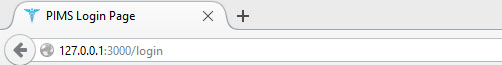
\includegraphics[width=\linewidth]{./Graphics/login.jpg}
\newline

Front end representation
\newline

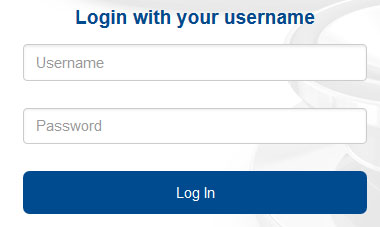
\includegraphics[width=\linewidth]{./Graphics/frontEnd.jpg}
		
User Authentication tested for the following conditions					
	\begin{itemize}
				\item Provide user with access
				\item Retrieve username
				\item Retrieve user password
				\item Fail with empty username and/ or empty password
				\item Return a boolean with regards to user right.
 \end{itemize}
 
 The figure bellow depics the successful testing of the Authentication and checkAdmin functions.
 \newline
 
 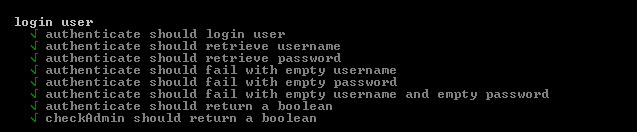
\includegraphics[width=\linewidth]{./Graphics/userResults.jpg}
 
 \subsubsection{Remarks}
 	\begin{itemize}
 				\item Pre-Conditions
 		User does not have access to systme.
 				\item Post-Conditions
 With correct login details, user successfuly gains access into the system with.
 User rights are checked upon login authentication
  \end{itemize}
  
  Both Pre and Post conditions  are considered in the implimentation of the system login. Unit testing successfuly.  tested with no violations to the security of the systm.
 
	\subsection{PIMS Notifications}
	%By Maria/
 \subsubsection{Pims Login}
Pims Send Notification is a two part function that we tested. First check if user is found(exists) in the database. Then send email using smtp.The unit test codes bellow demonstrates.
\newline

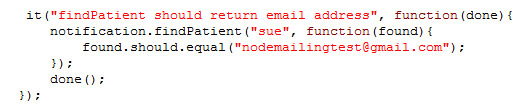
\includegraphics[width=\linewidth]{./Graphics/find.jpg}
\newline

Send Notifications via email
\newline

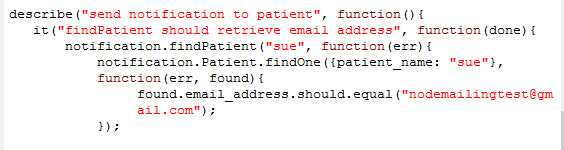
\includegraphics[width=\linewidth]{./Graphics/send.jpg}
The following conditions must be true for the send notification use case to pass.					
	\begin{itemize}
				\item Find patient should query the database to see if a user exists by searching for an email adress.
				\item Oce user is found, send notification must send and email to the found adress.
 \end{itemize}
 
 The figure bellow depics the successful testing of the Send Notification and FindUser functions.
 \newline
 
 \includegraphics[width=\linewidth]{./Graphics/Notify.jpg}
 
 \subsubsection{Remarks}
 	\begin{itemize}
 				\item Pre-Conditions
 		User must exist in database and have and email.
 				\item Post-Conditions
	User recieves and email from Prof Snyman.
  \end{itemize}
  
  Both Pre and Post conditions  are considered in the implimentation of sending notifications. Unit testing successfuly.  tested with no violations to the security of the systm.
 
	\subsection{PIMS Edit Profile}
	%By Maria/
 \subsubsection{Pims Login}
Pims edit user profile should be able to allow the admin user to update his profile and edit his information accordingly.
\newline

The Code bellow demonstrates the update of the user name after retrienving it.
\newline
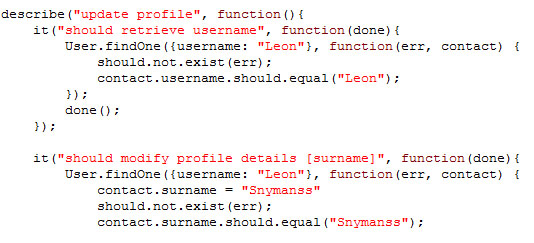
\includegraphics[width=\linewidth]{./Graphics/editCode.jpg}
\newline
		
Edit profile was  tested for the following conditions					
	\begin{itemize}
				\item Retrieve data
				\item Modify profile details
 \end{itemize}
 

 The figure bellow depics the successful testing of the UpdateAuthentication and checkAdmin functions.
 \newline
 
 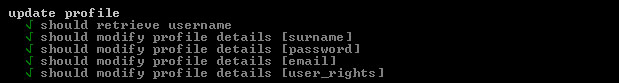
\includegraphics[width=\linewidth]{./Graphics/editProfile.jpg}

 
	\subsection{PIMS Add User}
	
Adding a user, is a feature only available for the admin user and is a crucial use-case needed for saving a new user’s to the system.
\newline
\newline
The add user case passed unit testing successfully as seen in the figure bellow
\newline
\newline
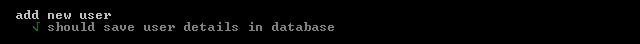
\includegraphics[width=350px]{./TestingDoc/Graphics/addUser}
\newline		
\subsubsection*{Conditions}
The following pre and post conditions are defined for adding a new user.
\newline
\newline	
\subsubsection*{Pre conditions}	
\begin{itemize}
		\item User must be logged in as admin.
		\item User to be added must not already exist in the database.
		\item User must be a medical personnel.
\end{itemize}	

\subsubsection*{Post conditions}	
\begin{itemize}
		\item New user is added and can interact with the system.
\end{itemize}	

The code bellow shows the testing for adding a new user with sample data	
\newline
\newline
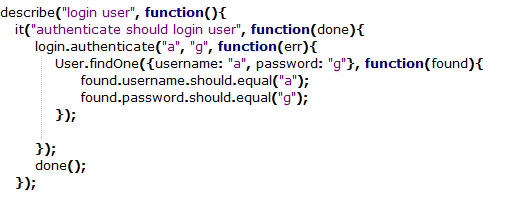
\includegraphics[width=350px]{./TestingDoc/Graphics/UserMustLogIn}

\subsubsection*{Remark}
Add User unit test successfully passes.
	\subsection{PIMS Statistics}
	%By Maria
\subsection{Login and Admnistartive user}
	\subsubsection*{PIMS Login}
		Functional Testing
		- for each use case tested
		* either success or a list of violations of the contract requirements (pre- and post-condition violations or data structure requirements)
		* a test coverage analysis reporting which percentage of the use cases have been covered by the testing
		
		2. Non-functional testing/assessment
		- any performance, scalability, maintainability, reliability, usability, ... problems identified with evidence for the identified problem.
	
				
					\begin{itemize}
							\item The Buzz Space system has to accommodate and host a multitude of users concurrently, thus making it prone to various malfunctions and glitches
							
							\item The Space needs to be monitored in real time at all times to ensure relevance of topics and subject matters.
							\item The rating and tagging functionality need to be fair and accurate
							
							\item Sufficient feedback and updates of the Buzz Space state must be provided to the users. Users that create threads or just comment on one.
							
							\item General software control and application usage..
						 \end{itemize}
	%\subsection{PIMS Artificial Inteligence}
	%\subsection{PIMS MyAdminSpace}
	%\subsection{PIMS MySpace}
	%\subsection{PIMSFORMS SaveForLater}
	%\subsection{PIMSFORMS SubmitForm}
	%\subsection{PIMSFORMS CancelForm}
	%\subsection{PIMSFORMS UpdateForm}
	
%\section{FEATURES NOT TO BE TESTED (Non-Functional Requirements)}
	%\subsection{Usability}
	%\subsection{Scalability}
	%\subsection{Performance}
	%\subsection{maintainability}
	%\subsection{Reliability}
	%\subsection{Secutity}
	%\subsection{Monitorability}
	%\subsection{Extendability}

%\section{APPROACH}
	%\subsection{Component Testing}
	%\subsection{Integration Testing}
	%\subsection{Conversion Testing}
	%\subsection{Job Stream Testing}
	%\subsection{Interface Testing}

	%\subsection{Recovery Testing}
	%\subsection{Performance Testing}
	%\subsection{Regression Testing}
	%\subsection{Acceptance Testing}
	
%\section{PASS / FAIL CRITERIA}
	%\subsection{Suspension Criteria}
	%\subsection{Resumption Criteria}
	%\subsection{Approval Criteria}
		
%\section{Testing Process}
	%\subsection{Test Deliverables}
	%\subsection{Testing Tasks}
	%\subsection{Responsibilities}
	%\subsection{Resources}
	%\subsection{Schedule}
	
%\section{Environmental Requirements}
	%\subsection{Hardware}
	%\subsection{Software}
	%\subsection{Security}
	%\subsection{Tools}
	%\subsection{Publications}
	%\subsection{Risks and Assumptions}

%\section{Change Management Procedures}

%\section{Remarks}
	%\subsection{Risks and issues}
	%\subsection{Product quality}
	%\subsection{Possible improvements}

%\section{Conclusion}

\newpage
\bibliographystyle{plain}
%include .bib file
\bibliography{./Architectural_Requirements/references}

\end{document}